\subsection{Choice of clocking rate}
After investigation of several papers on high-speed links, we have decided to use a half-rate clocking scheme. Several sources ~\cite{rajesh2011a} ~\cite{palermo2010a} ~\cite{cressler2007a} cite half-rate clocking as being more power efficient in terms of clock-generation and distribution than a full-rate clock, some of these papers also point out that the power burned in the transmitter multiplexer can be a problem when dealing with quarter-rate clocking or lower. One of the largest motivators for choosing half-rate clocking in the preliminary design is due to the graph in figure \ref{fig:graph}. In this graph the distribution of clocking-schemes across different bit-rates and clock-frequencies can be observed, and it is clear that at 10Gb/s the half- and full-rate clocking schemes are the most used.

\begin{figure}[ht!]
\begin{center}
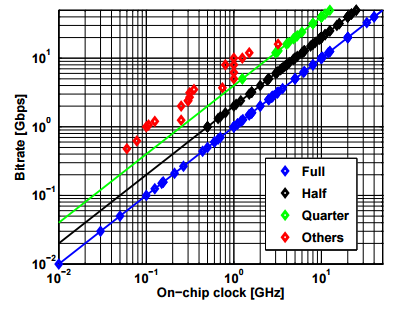
\includegraphics[scale=1.2]{img/clock0}
\caption{Use of different clock-rates in different implementations, source: ~\cite{rajesh2011a}}
\label{fig:graph}
\end{center}
\end{figure}

Taking a look at the graph in figure \ref{fig:graph1} the distribution of used clocking schemes in different technologies and their power consumption can be observed.

\begin{figure}[ht!]
\begin{center}
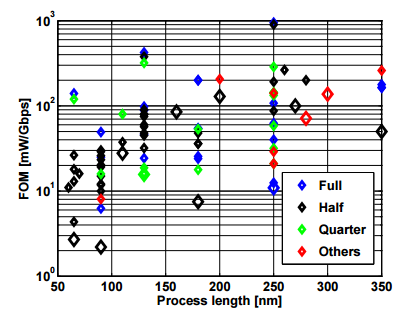
\includegraphics[scale=1.2]{img/clock1}
\caption{Distribution of different clock-rates in different technologies and their FOM, source: ~\cite{rajesh2011a}}
\label{fig:graph1}
\end{center}
\end{figure}

From the graph in figure \ref{fig:graph1} it can be observed that the half-rate clocking scheme is the most used in the 65nm process, and is also the clocking-rate that achieves the best power efficiency.

The half-rate clocking will be used at both the Tx and Rx side of the implementation in order to keep the design simple.